\documentclass[letterpaper]{article}
\usepackage{natbib,alifexi}
\usepackage[utf8]{inputenc}
\usepackage{amsmath}
\usepackage[toc,page]{appendix}
\usepackage[frenchb]{babel}
\usepackage[T1]{fontenc}
\usepackage{placeins, latexsym, amssymb}
\usepackage{comment}

\usepackage[hidelinks]{hyperref}

\title{Time stretching en temps réel pour le live coding}
\author{Abdeselam El-Haman Abdeselam$^{1}$\\
Superviseur : Bernard Fortz
\mbox{}\\\\
$^1$Université Libre de Bruxelles \\
aelhaman@ulb.ac.be}

%\setlength{\parskip}{0.5em}

\begin{document}
\maketitle

\begin{abstract}
  Overtone est une libraire en Clojure qui est utilisée pour faire du
  Live Coding (l'art de programmer en \og vif \fg{}). Une des techniques les
  plus utilisées dans le domaine de la musique synthétisée est le
  time-stretching, qui consiste à rallonger ou rétrécir une pièce musicale
  sans changer sa tonalité. Le time-stretching est intéressant dans
  le live-coding lorsqu'on peut modifier les paramétres de celui-ci
  en temps réel. Dans cet article 2 méthodes de time-stretching avec des
  approches différentes seront analysées, comparées et utilisées en temps
  réel dans Overtone.

\end{abstract}

\section{Introduction}

  Depuis le débuts de la musique éléctronique, le ``resampling'' de pièces musicales
  (c'est à dire, la manipulation de celles-ci) a un rôle important pour pouvoir manipuler
  des pièces musicales (rajouter des filtres, des envelopes, etc \ldots ) [rajouter citation ici].

  Un son est un signal qui est défini par sa durée, sa fréquence et son amplitude. La fréquence
  définit son ``pitch'' ou tonalité. La tonalité d'un son est plus grave si la fréquence est plus
  petite (donc une période plus grande).
  
  La manipulation d'un son dans le temps est utilisée très souvent lors du mixage et DJing.
  Ce genre de manipulations aident à rétrécir ou prolonger cette pièce pour, par exemple, mettre
  un son à la même vitesse que le ``tempo'' d'une chanson.

  Cette manipulation aura comme résultat aussi un effet sécondaire. La prolongation du signal
  provoquera aussi que la fréquence de ce signal soit modifié, et avec ça, un changement
  de tonalité non désiré se produira.

  \begin{figure}[h]
    \centerline{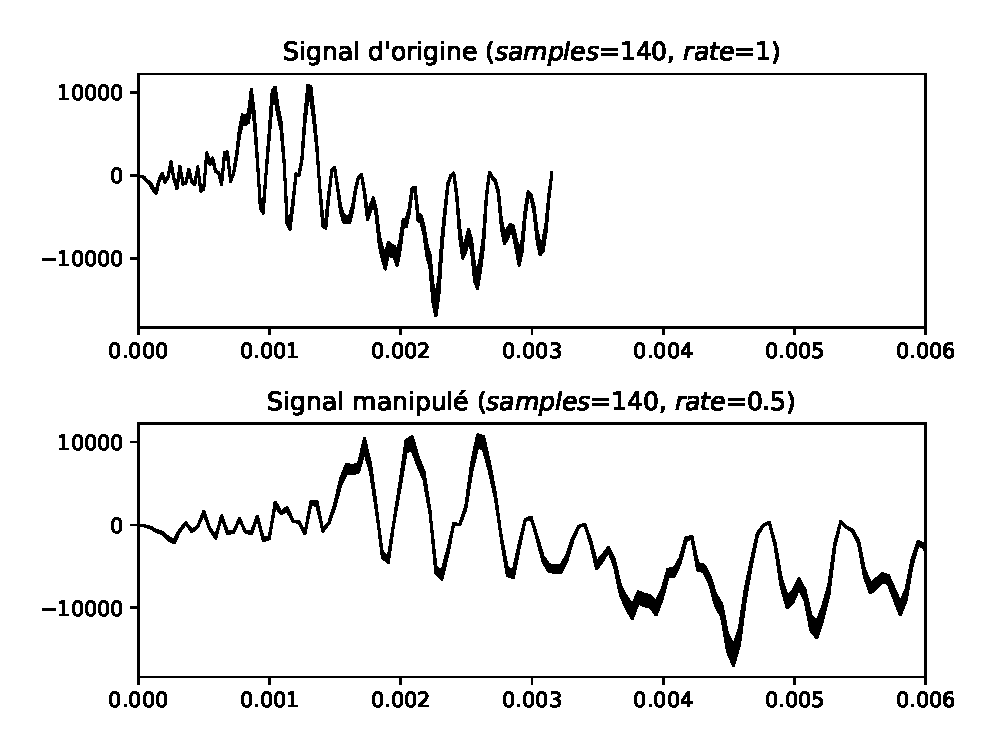
\includegraphics[width=9cm]{res/fig1.eps}}
    \caption{\label{fig:guitar-stretch}Sample d'une guitare lu à des vitesses différents}
  \end{figure}
  
  Le time-stretching est une technique pour éradiquer ce problème: changer le tempo d'un
  son sans changer sa tonalité.

  Plusieurs algorithmes existent pour implementer cette technique. Dans cet article l'état de
  l'art du time-stretching sera étudié et plusieurs de ces algorithmes seront
  implémentés pour l'application en temps réel de cette technique sur Overtone, une librairie pour
  qui a été conçue pour le traitement et synthèse de son. 



\begin{comment}
  Parler du son c'est quoi frequence etc

  C'est quoi le problème time stretching?
  À quoi est-il dû?
\end{comment}

\section{État de l'art}
\begin{comment}
  Techniques, un peu d'histoire?
\end{comment}

\subsection{Traitement du temps}
\begin{comment}
Parler de SOLA, PSOLA...
\end{comment}

\subsection{Traitement des fréquences}
\begin{comment}
  Parler du Vocodeur de phases, comment c'est utilisé etc...
\end{comment}
\subsection{Traitement du temps et des fréquences}
\begin{comment}
  On parle des techniques comme PVSOLA -> SOLA en prenant en compte la phase etc
\end{comment}

\section{Méthodes}

Les 2 méthodes qui ont été développées sont la granulation et le vocodeur de phases.
Ces 2 méthodes ont été utilisées en utilisant la fonction le système de génération de
synthétiseurs ``defsynth'' d'Overtone.
\begin{comment}
  Parler d'Overtone, Supercollider...
  UGENs qu'on va utiliser: PVRecordBuf, PVPlayBuf..
\end{comment}

\subsection{Langages fonctionnels}
\begin{comment}
\end{comment}

\subsection{Overtone}
\begin{comment}
  Parler d'Overtone-supercollider, les methodes que ça nous donne etc
  [CITER ARTICLE SONICPI -> OVERTONE DE SAM AARON]
\end{comment}

\subsection{AWESOME OVERTONE TWEAK THINGS}
\subsection{TD-SOLA}
\subsection{Vocodeur de phases}


\section{Résultats}

\section{Remerciements}
  Je remercie mon prometeur, Bernard Fortz, de m'avoir fait découvrir
  les yeux au monde du live-coding et la programmation fonctionnelle.

  Je tiens aussi à remercier l'UrLab pour m'avoir accueilli au SmartMonday
  pour partager avec eux tout ce que j'ai appris lors de mes recherches
  pour ce mémoire.

\footnotesize
\bibliographystyle{apalike}
\bibliography{rapport}


\end{document}
